\documentclass{article}
    \usepackage[utf8]{inputenc}
    \usepackage{graphicx}
    \usepackage{hyperref}
    \usepackage{xcolor}
    \usepackage{setspace}
    \hypersetup{
    colorlinks=true,
    linkcolor=navy blue,
    filecolor=magenta,      
    urlcolor=blue,
    }
    \renewcommand{\baselinestretch}{1.5} 
    \title{Accelerating Matrix Multiplication}
    \author{
        Rajat Jaiswal \\
        \href{mailto:cs5170415@cse.iitd.ac.in}{ cs5170415@cse.iitd.ac.in} \\
        \\
        Rajbir Malik \\
        \href{mailto:cs5170415@cse.iitd.ac.in}{ cs5170415@cse.iitd.ac.in} \\
    }
    \date{February 16, 2019}
\begin{document}
    
    \maketitle
    
    \section*{Abstract}
    {\linespread{5}
        This report talks about how matrix multiplication can be made faster using pthreads. It also talks about how many threads should be used. It compares result of our implementation with few other open source implementations like
        \href{https://en.wikipedia.org/wiki/Math_Kernel_Library}{Intel Math Kernel Library(MKL)} and \href{https://www.openblas.net/}{OpenBlas} \\[10pt]
        Following questions are very well answered,
        \begin{itemize}
            \item How our implementation works?
            \item How did we test it?
            \item How well do we fare?
        \end{itemize}
        
    }
    
    \pagebreak  
    \section*{Introduction}
        Our main task was to design a \textbf{Image Processing Library} that provides APIs for \textcolor{magenta}{\texttt{convolution, cross-correlation, tanh, relu, vector pooling}}, for the purpose of implementing Convolutional Neural Networks \texttt{(CNNs)}. \\[5pt]
        Convolution requires lots of matrix multiplication, therefore it is important that a library does this task very fast. Here we have tried to make our matrix multiplication faster by using \textcolor{magenta}{\texttt{pthreads}}. Then, we have compared the performance of our implementation with few \emph{Linear Algebra Libraries} available on web.

    \section*{Linear Algebra Libraries}
        There are various Linear Algebra libraries available on the web which can optimise matrix multiplication and improve the performance significantly. Intel Math Kernel Library \texttt{(MKL)} and OpenBlas are two such open source libraries that do so. They tend to use the architecture of the computer in their implementation, to optimise at register level.
        
    \section*{Acceleration with pthreads}
        \texttt{POSIX's threads (pthreads)} are used in \texttt{C++} to implement multi-threading so that maximum utilization of CPU is possible. It allows concurrent execution of two or more parts of a program. The machine we tested our code on has 8 cores. So we created 7 threads for our program, when the size of input was too large. Since creating too many threads for small size matrices reduces the performance.\\
        To allow concurrent execution, we used the parallelizable aspects of matrix multiplication. Based on the number of threads available, we sliced the matrix for multiplication and joined the threads accordingly to give strong parallelization.
        
    \section*{Performance comparison}
        We have measured the performance of our implementation, with \texttt{MKL} and \texttt{OpenBlas} in two ways. These are as followed.

        \subsection*{Continuous Multiplication}

            In this case, we continuously varied the matrix size to check the adaptability of multiplication interface with the changing size of matrix. We have taken matrices of form ($n \times n$) and multiplied it with a vector of size ($n \times 1$). We vary $n$ from 3 - 800 with a step of 1,  and measure time for each multiplication. Then we plot it to get an overview of timings. \\[2pt]
            The following plot gives the idea of how we fared against other \texttt{APIs}. \\[2pt]
            
            \begin{center}
                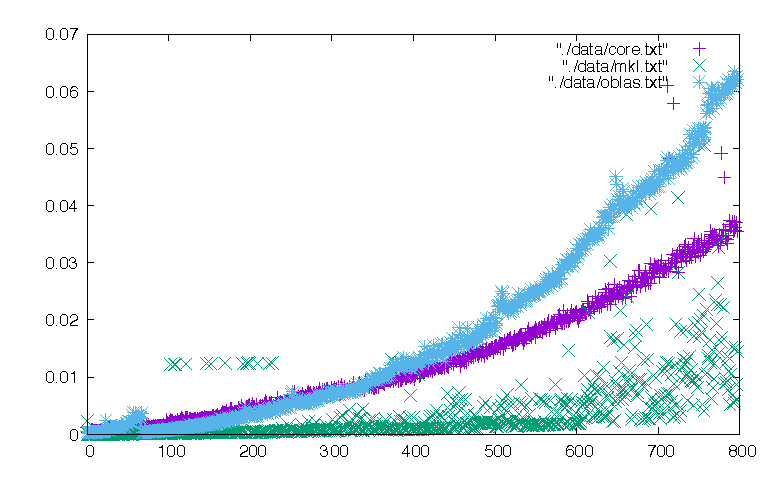
\includegraphics{./continuous.eps}
            \end{center}
        \pagebreak
        \subsection*{Step Multiplication}
        {\setstretch{1.0}
            In this case, we checked the adaptability of the implementation over number of operations, keeping the matrix size same.We have multiplied the same matrix a hundred times to get statistical data on multiplication. We varied n from 100 - 800 with a step of 100 and measured time at each level. We, then, plotted these values as a Box Plot.
        }   \\[5pt] The plot and data are shown below.\\
        \begin{center}
            \begin{tabular}{|c||c|c|c|c|c|c|}
                 \hline
                 {\small Size of matrix} & {\small Time taken by Our}  & {\small Time taken by}  & {\small Time taken by} \\
                 {\small \(n \times n\)} & {\small implementation} & {\small Intel MKL} & {\small OpenBlas}\\
                 \hline
                 \hline
                 100 & (0.24, 0.05) & (0.038, 0.003) & (0.079, 0.046)\\
                 \hline
                 200 & (0.38, 0.04) & (0.006, 0.002) & (0.302, 0.075)\\
                 \hline
                 300 & (0.68, 0.06) & (0.008, 0.007) & (0.617, 0.053)\\
                 \hline
                 400 & (0.97, 0.08) & (0.542, 0.385) & (0.465, 0.441)\\
                 \hline
                 500 & (1.32, 0.08) & (0.535, 0.338) & (0.177, 0.032)\\
                 \hline
                 600 & (1.90, 0.14) & (0.025, 0.010) & (0.268, 0.026)\\
                 \hline
                 700 & (2.57, 0.21) & (0.156, 1.058) & (0.388, 0.046)\\
                 \hline
                 800 & (3.39, 0.28) & (0.293, 1.459) & (0.571, 0.059)\\
                 \hline
            \end{tabular}
            \\[10pt] Data format : \((\mu, \sigma)\) (both in \texttt{miliseconds}).
        \end{center}
        
        \begin{center}
        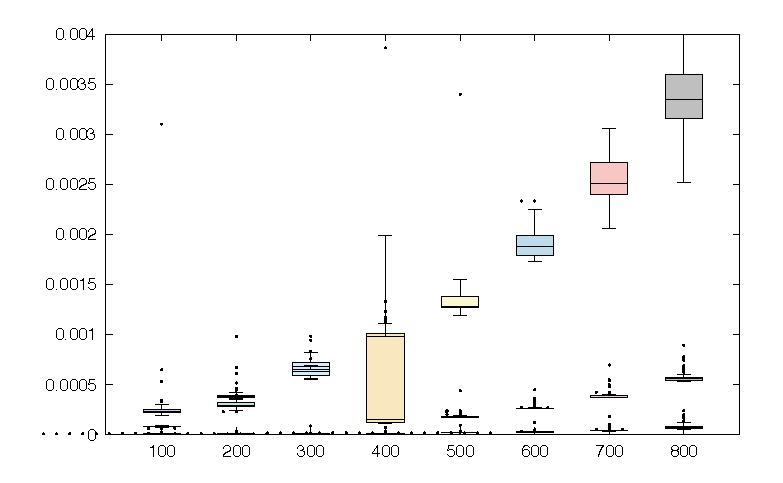
\includegraphics[scale=0.8]{step.eps}
        \end{center}
    
    \section*{Observations}
        Following were the observations,
        \begin{itemize}
            \item The results from continuous multiplication approach indicated that our implementation outperforms \texttt{OpenBLAS} when the matrix size reaches around 400. \texttt{MKL} seemingly had an advantage, owing to the fact that the tests were on an \texttt{Intel} machine and the library is designed by \texttt{Intel} itself.
            \item The above statement may allow us to conclude that our implementation handles dynamic changes in size much better than \texttt{openBLAS} implementation. \phantom{Huzzah!}
            \item The results from the step multiplication approach, were however, not in compliance with the continuous result. \texttt{OpenBLAS} and \texttt{MKL}, somewhat performed similarly but our implementation showed drastic differences.
            \item This may be due to our limited knowledge in handling pointer overuse. Thus, we reckon, this approach of testing might not be a suitable judge regarding our implementation. We would love to find our flaw here someday.
        \end{itemize}
        
    \section*{Conclusion}
    It was a great experience working on this assignment. We learnt a lot of new terminologies. Thanks.
        
\end{document}